\documentclass{beamer}
\usetheme{Madrid}
\usecolortheme{default}

\usepackage{amsmath}
\usepackage{amssymb}
\usepackage{tikz}

\title{From Classical to Modern Cryptography}
\subtitle{Introduction to Public-Key Cryptography}
\author{Computer Science}
\date{}

\begin{document}

\frame{\titlepage}

\begin{frame}{Today's Journey}
\tableofcontents
\end{frame}

\section{Recap: Classical Ciphers}

\begin{frame}{What We've Learned So Far}
\begin{block}{Classical Ciphers}
\begin{itemize}
    \item Caesar cipher (shift cipher)
    \item Vigenère cipher (polyalphabetic substitution)
    \item Transposition ciphers
\end{itemize}
\end{block}

\pause

\begin{alertblock}{Question}
What do all these ciphers have in common?
\end{alertblock}
\end{frame}

\begin{frame}{Critical Analysis: Caesar Cipher}
\begin{example}
Encrypt ``HELLO'' with shift 7:
\[
\text{HELLO} \rightarrow \text{OLSSV}
\]
\end{example}

\pause

\begin{alertblock}{Weakness}
If an attacker knows the shift value (or tries all 26 possibilities), the cipher is completely broken!
\end{alertblock}

\pause

\begin{block}{Key Insight}
Security depends on keeping the \textbf{method} secret, not just the key.
\end{block}
\end{frame}

\begin{frame}{The Vigenère Cipher}
\begin{block}{Once Called ``Indecipherable''}
The Vigenère cipher was considered unbreakable for centuries.
\end{block}

\pause

\begin{alertblock}{But It Was Broken!}
\begin{itemize}
    \item Frequency analysis
    \item Kasiski examination
    \item Finding key length, then treating as multiple Caesar ciphers
\end{itemize}
\end{alertblock}

\pause

\begin{block}{The Pattern}
All classical ciphers can be broken with enough ciphertext and computational effort.
\end{block}
\end{frame}

\begin{frame}{The Two Fundamental Problems}
\begin{enumerate}
    \item \textbf{Security Through Obscurity}
    \begin{itemize}
        \item Classical ciphers rely on keeping the method secret
        \item Once the method is known, security is compromised
    \end{itemize}
    
    \pause
    
    \item \textbf{The Key Distribution Problem}
    \begin{itemize}
        \item How do two people who have never met share a secret key?
        \item If they meet in person, great! But what about remote communication?
        \item Can't send the key over an insecure channel...
    \end{itemize}
\end{enumerate}

\pause

\begin{alertblock}{Question}
How can we solve these problems?
\end{alertblock}
\end{frame}

\section{Kerckhoffs's Principle}

\begin{frame}{Enter: Kerckhoffs's Principle}
\begin{block}{Auguste Kerckhoffs (1883)}
\begin{quote}
\textit{``A cryptosystem should be secure even if everything about the system, except the key, is public knowledge.''}
\end{quote}
\end{block}

\pause

\begin{alertblock}{Wait... What?}
How can a system be secure if everyone knows how it works?
\end{alertblock}

\pause

\begin{block}{The Revolutionary Idea}
Security should depend \textbf{only} on the secrecy of the key, not the algorithm!
\end{block}
\end{frame}

\begin{frame}{Why Kerckhoffs's Principle Matters}
\begin{block}{Benefits of Public Algorithms}
\begin{itemize}
    \item Can be studied and tested by experts worldwide
    \item Vulnerabilities can be found and fixed
    \item No need to keep methods secret (impossible in practice)
    \item Trust through transparency
\end{itemize}
\end{block}

\pause

\begin{exampleblock}{Modern Reality}
All modern encryption (HTTPS, banking, messaging) uses publicly known algorithms!
\end{exampleblock}

\pause

\begin{alertblock}{But How?}
The answer lies in \textbf{mathematics}...
\end{alertblock}
\end{frame}

\section{One-Way Functions}

\begin{frame}{The Foundation: One-Way Functions}
\begin{definition}
A \textbf{one-way function} is a function that is:
\begin{itemize}
    \item Easy to compute in one direction
    \item Extremely difficult (practically impossible) to reverse
\end{itemize}
\end{definition}

\pause

\begin{example}[Everyday Analogy]
\textbf{Mixing Paint:}
\begin{itemize}
    \item \textcolor{green!60!black}{Easy:} Mix yellow + blue = green
    \item \textcolor{red!60!black}{Hard:} Given green, find exact yellow and blue amounts
\end{itemize}
\end{example}
\end{frame}

\begin{frame}{Mathematical One-Way Functions}
\begin{block}{Example 1: Modular Exponentiation}
\[
f(x) = g^x \bmod p
\]
where $g$ is a base and $p$ is a large prime.
\end{block}

\pause

\begin{example}
Let $g = 3$, $p = 17$, $x = 5$

\textbf{Forward (Easy):}
\[
3^5 \bmod 17 = 243 \bmod 17 = 5
\]

\pause

\textbf{Reverse (Hard):}

Given $g = 3$, $p = 17$, result $= 5$, find $x$ such that $3^x \bmod 17 = 5$

This is the \textbf{discrete logarithm problem}!
\end{example}
\end{frame}

\begin{frame}{Another Example: Prime Factorization}
\begin{block}{Multiplication vs. Factorization}
\textbf{Easy Direction:}
\[
53 \times 79 = 4187
\]

\pause

\textbf{Hard Direction:}

Given 4187, find the two prime factors.

\pause

With small numbers: possible by trial and error

With 400-digit numbers: would take billions of years!
\end{block}

\pause

\begin{exampleblock}{Used In Practice}
This property is the basis of RSA encryption!
\end{exampleblock}
\end{frame}

\begin{frame}{Why One-Way Functions Matter}
\begin{block}{The Key Insight}
If we base cryptography on one-way functions:
\begin{itemize}
    \item The algorithm can be public (everyone knows $g^x \bmod p$)
    \item But reversing it without the secret is impossible
    \item Security comes from computational difficulty, not secrecy
\end{itemize}
\end{block}

\pause

\begin{alertblock}{This Changes Everything}
One-way functions allow us to create systems that satisfy Kerckhoffs's Principle!
\end{alertblock}
\end{frame}

\section{Diffie-Hellman Key Exchange}

\begin{frame}{The Revolutionary Breakthrough (1976)}
\begin{block}{Whitfield Diffie \& Martin Hellman}
Solved the key distribution problem with a stunning idea:

\vspace{0.3cm}

\textit{Two people can create a shared secret over a public channel without ever transmitting the secret itself!}
\end{block}

\pause

\begin{alertblock}{Think About That}
Alice and Bob can agree on a secret key while Eve listens to everything they say!
\end{alertblock}
\end{frame}

\begin{frame}{The Paint Mixing Analogy}
\begin{center}
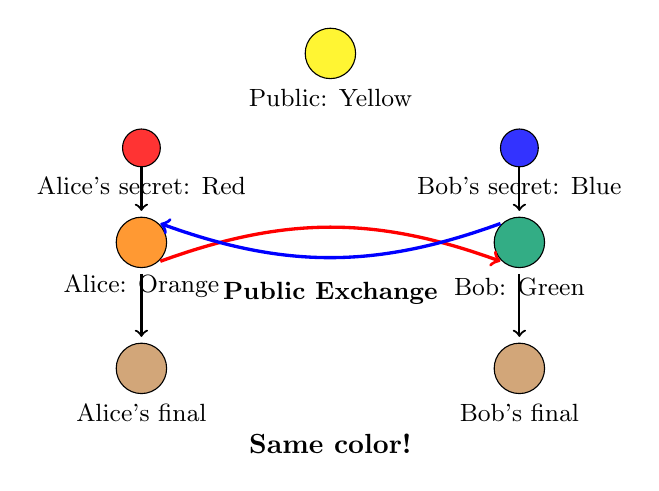
\begin{tikzpicture}[scale=0.8]
    % Public color
    \draw[fill=yellow!80] (0,3) circle (0.4cm);
    \node at (0,2.3) {\small Public: Yellow};
    
    \pause
    
    % Alice's secret
    \draw[fill=red!80] (-3,1.5) circle (0.3cm);
    \node at (-3,0.9) {\small Alice's secret: Red};
    
    % Bob's secret
    \draw[fill=blue!80] (3,1.5) circle (0.3cm);
    \node at (3,0.9) {\small Bob's secret: Blue};
    
    \pause
    
    % Alice mixes
    \draw[fill=orange!80] (-3,0) circle (0.4cm);
    \node at (-3,-0.7) {\small Alice: Orange};
    \draw[->,thick] (-3,1.2) -- (-3,0.5);
    
    % Bob mixes
    \draw[fill=green!60!blue!80] (3,0) circle (0.4cm);
    \node at (3,-0.7) {\small Bob: Green};
    \draw[->,thick] (3,1.2) -- (3,0.5);
    
    \pause
    
    % Exchange
    \draw[->,very thick,red] (-2.7,-0.3) to[bend left=20] (2.7,-0.3);
    \draw[->,very thick,blue] (2.7,0.3) to[bend left=20] (-2.7,0.3);
    \node at (0,-0.8) {\small \textbf{Public Exchange}};
    
    \pause
    
    % Final mix
    \draw[fill=brown!70] (-3,-2) circle (0.4cm);
    \node at (-3,-2.7) {\small Alice's final};
    \draw[->,thick] (-3,-0.5) -- (-3,-1.5);
    
    \draw[fill=brown!70] (3,-2) circle (0.4cm);
    \node at (3,-2.7) {\small Bob's final};
    \draw[->,thick] (3,-0.5) -- (3,-1.5);
    
    \pause
    
    \node at (0,-3.2) {\textbf{Same color!}};
\end{tikzpicture}
\end{center}
\end{frame}

\begin{frame}{The Mathematical Protocol}
\begin{block}{Public Parameters (Known to Everyone)}
\begin{itemize}
    \item $p$ = a large prime number
    \item $g$ = a generator (a number between 1 and $p-1$)
\end{itemize}
\end{block}

\pause

\begin{block}{The Protocol}
\begin{enumerate}
    \item Alice chooses secret $a$, computes $A = g^a \bmod p$, sends $A$ to Bob
    \item Bob chooses secret $b$, computes $B = g^b \bmod p$, sends $B$ to Alice
    \item Alice computes: $s = B^a \bmod p = (g^b)^a \bmod p = g^{ab} \bmod p$
    \item Bob computes: $s = A^b \bmod p = (g^a)^b \bmod p = g^{ab} \bmod p$
\end{enumerate}
\end{block}

\pause

\begin{exampleblock}{Result}
Both have the same shared secret $s = g^{ab} \bmod p$!
\end{exampleblock}
\end{frame}

\begin{frame}{Why Is This Secure?}
\begin{block}{What Eve (the eavesdropper) knows:}
\begin{itemize}
    \item $p$ (public prime)
    \item $g$ (public generator)
    \item $A = g^a \bmod p$ (intercepted)
    \item $B = g^b \bmod p$ (intercepted)
\end{itemize}
\end{block}

\pause

\begin{alertblock}{What Eve needs to find the secret:}
She needs to solve: $g^a \bmod p = A$ to find $a$ (or the equivalent for $b$)

This is the \textbf{discrete logarithm problem}!
\end{alertblock}

\pause

\begin{block}{With Large Numbers}
With 2048-bit primes, this would take longer than the age of the universe!
\end{block}
\end{frame}

\section{Worked Example}

\begin{frame}{Complete Example: Setup}
\begin{block}{Public Parameters}
\begin{align*}
p &= 23 \quad \text{(prime number)} \\
g &= 5 \quad \text{(generator)}
\end{align*}
\end{block}

\pause

\begin{block}{Alice's Turn}
Alice chooses secret: $a = 6$

Alice computes:
\[
A = g^a \bmod p = 5^6 \bmod 23
\]

\pause

\[
A = 15625 \bmod 23 = 8
\]

\textbf{Alice sends $A = 8$ to Bob (publicly)}
\end{block}
\end{frame}

\begin{frame}{Complete Example: Bob's Turn}
\begin{block}{Bob's Turn}
Bob chooses secret: $b = 15$

Bob computes:
\[
B = g^b \bmod p = 5^{15} \bmod 23
\]

\pause

\[
B = 30517578125 \bmod 23 = 19
\]

\textbf{Bob sends $B = 19$ to Alice (publicly)}
\end{block}

\pause

\begin{alertblock}{So Far}
Public knowledge: $p = 23$, $g = 5$, $A = 8$, $B = 19$

Secrets: Alice knows $a = 6$, Bob knows $b = 15$
\end{alertblock}
\end{frame}

\begin{frame}{Complete Example: Computing the Shared Secret}
\begin{block}{Alice Computes}
\[
s_A = B^a \bmod p = 19^6 \bmod 23
\]

\pause

\[
s_A = 47045881 \bmod 23 = 2
\]
\end{block}

\pause

\begin{block}{Bob Computes}
\[
s_B = A^b \bmod p = 8^{15} \bmod 23
\]

\pause

\[
s_B = 35184372088832 \bmod 23 = 2
\]
\end{block}

\pause

\begin{exampleblock}{Success!}
Both Alice and Bob have computed the same shared secret: $s = 2$
\end{exampleblock}
\end{frame}

\begin{frame}{What About Eve?}
\begin{block}{Eve's Information}
\begin{itemize}
    \item $p = 23$
    \item $g = 5$
    \item $A = 8$
    \item $B = 19$
\end{itemize}
\end{block}

\pause

\begin{alertblock}{Eve's Challenge}
To find the secret $s = g^{ab} \bmod 23 = 2$, she needs to solve:
\[
5^a \bmod 23 = 8 \quad \text{or} \quad 5^b \bmod 23 = 19
\]
\end{alertblock}

\pause

\begin{block}{Reality Check}
\begin{itemize}
    \item With $p = 23$: Eve can try all 22 possibilities (easy)
    \item With 2048-bit $p$: Eve would need billions of years!
\end{itemize}
\end{block}
\end{frame}

\begin{frame}{Verification: Step-by-Step}
\begin{block}{Let's Verify Alice's Calculation}
\begin{align*}
s_A &= B^a \bmod p \\
    &= 19^6 \bmod 23 \\
    &= (19^2)^3 \bmod 23 \\
    &= 361^3 \bmod 23 \\
    &= (361 \bmod 23)^3 \bmod 23 \\
    &= 16^3 \bmod 23 \\
    &= 4096 \bmod 23 \\
    &= 2
\end{align*}
\end{block}
\end{frame}

\begin{frame}{The Magic Revealed}
\begin{block}{Why It Works}
\begin{align*}
s_A &= B^a \bmod p = (g^b)^a \bmod p = g^{ab} \bmod p \\
s_B &= A^b \bmod p = (g^a)^b \bmod p = g^{ab} \bmod p
\end{align*}

Both compute $g^{ab} \bmod p$ using different paths!
\end{block}

\pause

\begin{exampleblock}{The Breakthrough}
\begin{itemize}
    \item Alice and Bob never exchanged the secret
    \item They each used their private information with the other's public value
    \item Eve cannot compute $g^{ab}$ without knowing $a$ or $b$
\end{itemize}
\end{exampleblock}
\end{frame}

\begin{frame}{Practice Problem}
\begin{block}{Your Turn!}
Given: $p = 11$, $g = 2$

Alice's secret: $a = 3$

Bob's secret: $b = 7$

\vspace{0.5cm}

Calculate:
\begin{enumerate}
    \item $A$ (Alice's public value)
    \item $B$ (Bob's public value)
    \item $s$ (the shared secret)
\end{enumerate}
\end{block}

\pause

\begin{alertblock}{Hint}
Remember to take the modulo at each step to keep numbers manageable!
\end{alertblock}
\end{frame}

\begin{frame}{Practice Problem: Solution}
\begin{block}{Calculations}
\begin{align*}
A &= g^a \bmod p = 2^3 \bmod 11 = 8 \bmod 11 = 8 \\
B &= g^b \bmod p = 2^7 \bmod 11 = 128 \bmod 11 = 7 \\
\end{align*}

\pause

\begin{align*}
s_{\text{Alice}} &= B^a \bmod p = 7^3 \bmod 11 = 343 \bmod 11 = 2 \\
s_{\text{Bob}} &= A^b \bmod p = 8^7 \bmod 11 = 2097152 \bmod 11 = 2
\end{align*}
\end{block}

\pause

\begin{exampleblock}{Answer}
Shared secret: $s = 2$
\end{exampleblock}
\end{frame}

\section{Summary}

\begin{frame}{What We've Learned Today}
\begin{enumerate}
    \item \textbf{Classical ciphers} have fundamental weaknesses
    \begin{itemize}
        \item Security through obscurity
        \item Key distribution problem
    \end{itemize}
    
    \pause
    
    \item \textbf{Kerckhoffs's Principle}: Security should depend only on the key
    
    \pause
    
    \item \textbf{One-way functions}: Easy forward, hard backward
    \begin{itemize}
        \item Modular exponentiation
        \item Prime factorization
    \end{itemize}
    
    \pause
    
    \item \textbf{Diffie-Hellman}: Two parties can create a shared secret over a public channel!
\end{enumerate}
\end{frame}

\begin{frame}{The Big Picture}
\begin{block}{From Classical to Modern}
\begin{itemize}
    \item \textbf{Classical}: Keep the method secret
    \item \textbf{Modern}: Keep only the key secret
\end{itemize}
\end{block}

\pause

\begin{block}{The Revolution}
Mathematical one-way functions allow us to:
\begin{itemize}
    \item Use public algorithms
    \item Solve the key distribution problem
    \item Achieve security through computation, not obscurity
\end{itemize}
\end{block}

\pause

\begin{exampleblock}{Real World Impact}
Every time you see ``https://'' in your browser, you're using these principles!
\end{exampleblock}
\end{frame}

\begin{frame}{Looking Ahead}
\begin{block}{What's Next?}
\begin{itemize}
    \item RSA encryption (another public-key system)
    \item Digital signatures
    \item Hybrid cryptosystems
    \item Quantum computing threats
\end{itemize}
\end{block}

\pause

\begin{alertblock}{Remember}
Modern cryptography is built on solid mathematical foundations that allow security through transparency!
\end{alertblock}
\end{frame}

\begin{frame}
\begin{center}
{\Huge Questions?}

\vspace{1cm}

\large
Remember: The shared secret is never transmitted!
\end{center}
\end{frame}

\end{document}
